%!TEX root=../document.tex



\section{Was ist Load Balancing?}\cite{Lastverteilung}
Der Begriff Load Balancing (zu deutsch Lastverteilung) beschreibt umfangreiche Berechnungen oder große Mengen von Anfragen, welche auf mehrere parallel arbeitende System verteilt werden. Es gibt verschiedene Ausprägungen, welche mit der Menge* der Kommunikation skalieren. Diese reichen von
Lastverteilung auf einem System mit mehreren Prozessoren, bis hin zu ganzen Computer-Clustern, welche die Arbeit auf mehrere Rechner aufteilen.

\section{Serverlastverteilung}

Serverlasterverteilung (englisch Server Load Balancing ''SLB'') kommt überall dort zum Einsatz, wo sehr viele Clients eine hohe Anfragedichte erzeugen und damit einen einzelnen Server-Rechner überlasten würden.\newline

Typische Kriterien zur Ermittlung der Notwendigkeit von SLB sind die \textbf{Datenrate}, die \textbf{Anzahl der Clients} und die \textbf{Anfragerate}. \newline

Die Erhöhung der Datenverfügbarkeit wird durh SLB gefördert. Reduntate Datenhaltung wird durh das Einsetzen von mehreren Systemen ermöglicht. Die Aufgabe des SLB ist hier die Vermittlung der Clients an die einzelnen Server. \newline

\section{Verfahren von SLB}
Es bieten sich einige verschiedene Verfahren, welche bei Server Load Balancing zum Einsatz kommen können. Ein mögliches Verfahren wäre das Vorschalten eines Systems (\textbf{Load Balancer, Frontend Server}), der Anfragen aufteilt, oder die Verwendung von DNS (Domain-Name-System) mit dem sogenannten \textbf{Round-Robin-Verfahren}. Bei Webservern darf eine Serverlastverteilung nicht fehlen, da ein einzelner Host nur eine begrenzte Anzahl an HTTP-Anfragen auf einmal beantworten kann. Es besteht auch die Möglichkeit, dass der Load Balancer die Verschlüsselung zum Client übernimmt und intern die Anfragen auf seine Art und Weiße verarbeitet. \newline

Es bestehen folgende Verfahren:
\begin{itemize}
	\item DNS Round Robin
	\item NAT based SLB
	\item Flat based SLB
	\item Anycast SLB
\end{itemize}

\newpage
\subsection{DNS Round Robin}\cite{LastverteilungPerDNS}


Lastverteilung per DNS (englisch Round robin DNS) ist die einfachste Technik zur SLB auf Basis des DNS. Da es aber zu einem Caching der DNS-Antworten kommt, ist dieses Verfahren nur manchmal wirklich sinnvoll.

\subsubsection{Aufbau und Funktionsweise}\cite{RoundRobinDNS}
DNS lässt es zu, dass einem Namen mehrere IP-Adressen zugewiesen werden können. Dies bedeutet es können mehrere sogenannte \textbf{Resource Records} mit gleichem Label, gleicher Klasse und gleichem Typ entstehen. Eine deartige Anordnung wird als \textit{Resource Record Set} bezeichnet.

\begin{figure}[!h]
	\begin{center}
		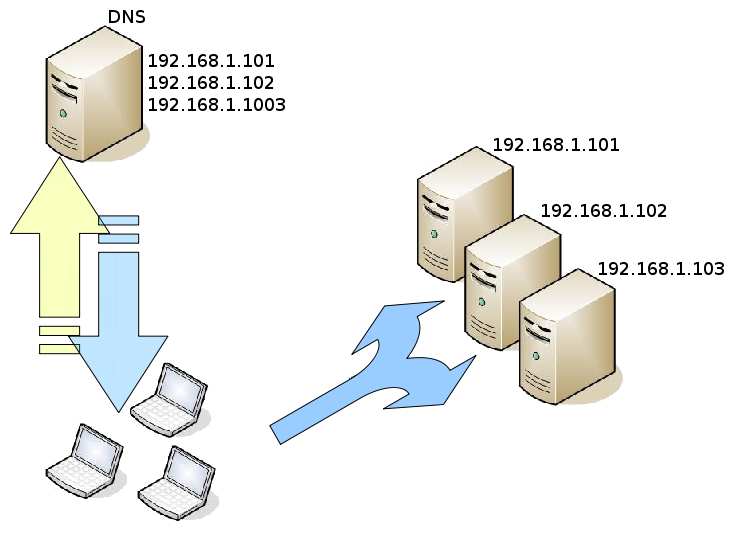
\includegraphics[width=0.5\linewidth]{images/RR-DNS}
		\caption{Grafik eines Aufbaus von DNS Round Robin}
		\label{broker}
	\end{center}
\end{figure}
\begin{center}

\begin{lstlisting}[caption=DNS Round Robin Example]
    server.example.com.   1800  IN  A  192.168.1.101
    server.example.com.   1800  IN  A  192.168.1.102
    server.example.com.   1800  IN  A  192.168.1.103
\end{lstlisting}
\end{center}
Wird ein derartiger Name von einem Resolver abgefragt, so liefert der DNS-Server grundsätzlich alle bekannten IP-Adressen zurück, allerdings in wechselnder Reihenfolge. Der erste Request wird dann beispielsweise mit [10.0.2.70, 10.0.2.71, 10.0.2.72] beantwortet und der zweite mit [10.0.2.71, 10.0.2.72, 10.0.2.70]. Der Resolver legt dann fest welche IP-Adresse verwendet werden soll.


Nach welcher Vorgangsweise ein DNS die Reihenfolge vorgibt, kann bei
\textit{Bind}-kompatiblen Nameservern konfiguriert werden. Bei \textbf{BIND} sind drei Varianten möglich: \textbf{zyklisch}, \textbf{zufällig} oder \textbf{fest}. Die Reihenfolge bei zyklisch und zufällig ist selbsterklärend, jedoch bei fest werden die IP-Adressen in der Reihenfolge zurückgegeben, in der sie im DNS abgelegt worden sind.

\subsubsection{Technischer Fortschritt}\cite{SRVResourceRecord}
Mittels \textbf{SRV} (Service Resource Records) kann per DNS erkannt werden, welche IP-basierenden Dienste in einer Domain angeboten werden. So wird zu jedem Dienst weitere Information geliefert, wie zum Beispiel der Sever-Name, der diesen Dienst bereitstellt.

\begin{center}
	
	\begin{lstlisting}[caption=SRV - (Service) Resource Records]
	_ldap._tcp.example.com. 3600  IN  SRV  10  0  389  ldap01.example.com.
	\end{lstlisting}
\end{center}


Bei \textbf{NAPTR}, ausgeschrieben \textit{Naming Authority Pointer Resource Records}
werden DNS-Namen, Adressen von Servern und weitere Informationen zugeordnet. Diese Records liefern die zusätzliche Informationen auf flexible Art und Weise. Außerdem wird das Protokoll angegeben, das der Server verwendet. Falls mehrere NAPTR-Records zu einem Namen existieren, kann eine \textbf{Priorisierung} festgelegt werden. Auch wenn mehrere Records gleicher Priorität zu einem Namen existieren, kann eine Lastverteilung erreicht werden.

Bei moderneren Resource-Record-Typen lässt sich außerdem noch eine Gewichtung definieren, die festlegt, welche Server-IP-Adressen am häufigsten an erster Stelle stehen. Die entsprechenden Server werden damit häufiger angesprochen.

Außerdem gibt es die Möglichkeit, aus einem Pool von möglichen Servern nur einige zurückzuliefern. So werden beispielsweise vom Google-Nameserver immer drei IP-Adressen zurückgeliefert, die teilweise wechseln. Sinnvoll ist auch eine standortbezogene Rücklieferung von IP-Adressen, wenn mehrere verteilte Rechenzentren zur Verfügung stehen.

\subsubsection{Nachteile}
Die Lastverteilung durch DNS ist natürlich nur in dem Sinn gleichmäßig, was die Zuteilung betrifft. Über die danach entstehende tatsächliche Belastung weiß DNS nichts. Auch wird nicht überprüft, ob die Zielserver überhaupt ansprechbar sind. Vorgeschaltete Skripts können aber die Verfügbarkeit prüfen und nur diejenigen Server im Nameserver eintragen, die aktuell tatsächlich zur Verfügung stehen. Damit lassen sich Lastverteilung und Ausfallsicherung verbinden.


\newpage

\subsection{Flat based SLB}

Bei diesem Verfahren wird nur ein Netzwerk benötigt. Die Server und der Load Balancer müssen über einen Switch miteinander verbunden sein. Sendet der Client eine Anfrage (an den Load Balancer), wird der entsprechende Ethernet-Frame so manipuliert, dass es eine direkte Anfrage des Clients an den Server darstellt.

\subsubsection{Aufbau und Funktionsweise}
Bei einer \textbf{flat based SLB}  tauscht der Load Balancer bei Anfragen seine eigene \textbf{MAC-Adresse} gegen die des zu vermittelnden Servers aus und sendet dann das Paket weiter. Die \textbf{IP-Adressen} bleiben hierbei \textbf{unverändert}. Bei einem deartigen Vorgehen spricht man auch von \textbf{MAT (MAC Address Translation)}. Der Server, welcher die Anfrage bekommen hat, schickt seine Antwort direkt an die IP-Adresse des Absenders, also die des Clients.

Der Client hat damit den Eindruck mit, er kommuniziere nur mit einem einzigen Rechner, welcher aber der Load Balancer ist, obwohl der Server selber tatsächlich nur mit einem einzigen Client kommuniziert. Dieses Verfahren wird als \textbf{DSR (Direct Server Return)} bezeichnet.

\begin{figure}[!h]
	\begin{center}
		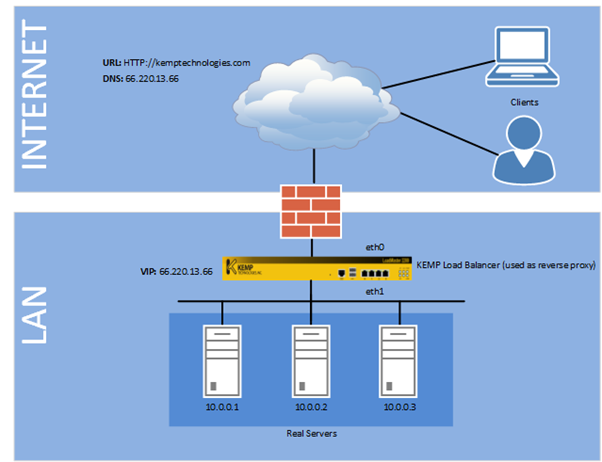
\includegraphics[width=0.5\linewidth]{images/flat_slb}
		\caption{Flat based SLB Architektur }
		\label{flat_based_SLB}
	\end{center}
\end{figure}

\subsubsection{Vorteile}
Der Vorteil bei Flat based SLB ist die Entlastung des Load Balancers, da der meist datenreiche Rückverkehr auf direktem Weg stattfindet.

\newpage
\subsection{NAT based SLB}\cite{SLBbook}

NAT basierte SLB-Netzwerkarchitekturen sind definitionsgemäß, jene Verfahren bei denen sich die IPs der \textbf{virtuellen IPs} und der \textbf{realen Server} in verschiedenen Subnets befinden. Diese Vorgänge heißen NAT, weil der Load Balancer NAT-Pakete zwischen zwei Subnets, wie eine \textbf{Firewall} oder ein \textbf{Router}, transferiert.

\subsubsection{Implementation}
Der Hauptunterschied zwischen NAT- und Flat-basierten Architekturen besteht darin, dass der Load Balancer ein NAT zwischen einem Netzwerk und einem anderen ausführt. Die wohl einfachste und typische Art, ein NAT based SLB zu implementieren, ist eine 
\textbf{route-path, two-armed} Konfiguration. In der \textbf{\hyperref[nat_slb_01]{nachfolgenden Abbildung}} wird der Ablauf so einer Konfiguration beschrieben. Es zeigt wie der Load Balancer die normalen \textbf{Routing-IP-Adressen} in \textbf{nonrouted} IPs, auf denen die realen Server sitzen, übersetzt.
\begin{figure}[!h]
	\begin{center}
		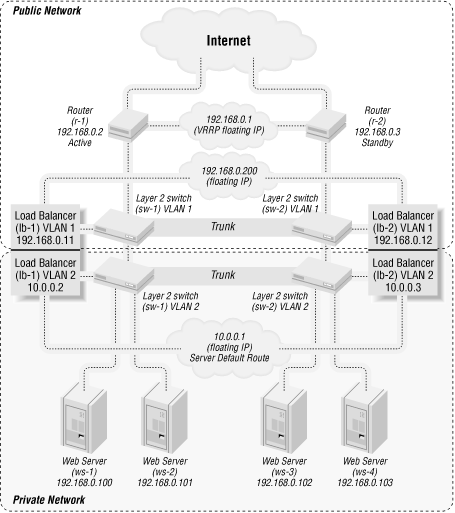
\includegraphics[width=0.5\linewidth]{images/slb_0701}
		\caption{route-path, two-armed Architektur}
		\label{nat_slb_01}
	\end{center}
\end{figure}
\newline
In dieser Konfiguration befinden sich die Server in einem separaten VLAN, welche die die VIP-Adressen (Virtuelle IP-Adressen) des Load Balancers besitzen. Die einzigen \textbf{floating IPs} befinden sich im \textit{public} Netzwerk, welche zwischen den \textbf{aktiven} und \textbf{standby} Load Balancern angelegt sind. Ein Floating-Standard-Gateway wird im \textit{public}-Bereich nicht benötigt, da die Load Balancer nicht die Rolle eines Gateways übernehmen. Das Floating-Gateway ist in das private Netzwerk integriert. Die Load Balancer bei diesem Verfahren die Rolle einer \textbf{Firewall} übernehmen, weil diese eine enge Kontrolle über den Netzwerkverkehr haben.

Außerdem gibt es noch eine andere Methode, bei der sich alle Geräte nur \textbf{ein LAN} teilen. Die Load Balancer sind hierbei für mehrere Netzwerke im selben LAN konfiguriert und übernehmen somit das NAT. In der \textbf{\hyperref[nat_slb_02]{folgenden Abbildung}} wird der Aufbau eines \textbf{route-path, one-armed} SLB dargestellt.
\begin{figure}[!h]
	\begin{center}
		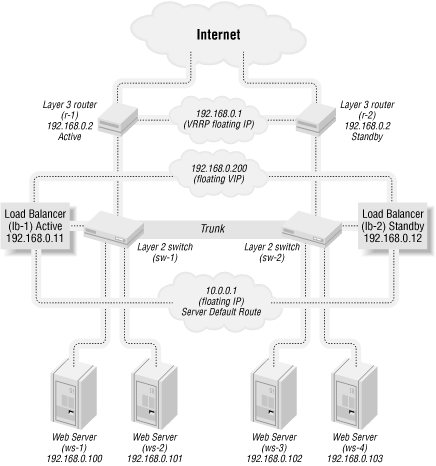
\includegraphics[width=0.5\linewidth]{images/slb_0702}
		\caption{route-path, one-armed Architektur}
		\label{nat_slb_02}
	\end{center}
\end{figure}

Die Load Balancer sind in dieser Architektur für zwei Subnetze im gleichen LAN konfiguriert, einer für die öffentlichen Schnittstellen der virtuellen IPs und der andere für das private Subnet der Server. Obwohl sich alles noch in einem LAN befindet, übernimmt der Load Balancer das NAT.

Sowohl aus Sicherheitsgründen als auch aus architektonischer Sicht ist es \textbf{besser}, eine \textbf{two-armed} Architektur mit zwei seperaten LANs (oder VLANs) zu verwenden. Wenn alles in ein LAN untergbracht wird, werden Sicherheitsziele und Vorteiler einer NAT-basierten Konfiguration vernachlässigt. Das tatsächliche Bestehen einer Schranke zwischen dem öffentlichen und privaten Netzwerk, verstärkt die Gesamtsicherheit eines Netzwerks. Der Datenfluß ist mit zwei VLANs einfach zu verwalten, da es klare Abgrenzungspunkte für die beiden getrennten Netze gibt, wodurch die Fehlersuche in den meisten Fällen extrem erleichtert wird.
\newpage

\subsubsection{Bridge-Path and Direct Server Return}
Da NAT von einem Netzwerk zu einem anderen eine Layer 3 Funktion im  OSI-Modell ist, st die Variante \textbf{bridge-path} keine Option für NAT-basiertes SLB. Damit NAT funktioniert muss der Load Balancer Interfaces auf zwei Netzwerken haben, aber bridge-path baut normalerweise auf nur einem Netz auf.

\textbf{DSR (Direct Server Return)} tritt nicht häufig, so wie bei flat-basierenden Architekturen, bei NAT-basierenden Szenarien auf, ist aber trotzdem möglich. Hiebei wird aber zusätzlich zum Load Balancer und einer Layer 2 Infrastruktur ein Layer 3 Gerät benötigt. Bei Direct Server Return werden Pakete bereits modifiziert versendet und das Layer 3 Element leitet diese einfach von einem Netzwerk zu einem anderen. Das Modifizieren benötigt zwar mehr Rechenleistung für die Server, ist aber eine Entlastung für den Load Balancer. In der \textbf{\hyperref[nat_slb_03]{folgenden Abbildung}} wird ein Beispiel einer solchen Konfiguration dargestellt.
\begin{figure}[!h]
	\begin{center}
		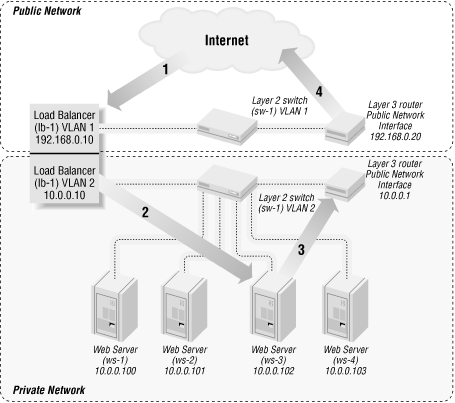
\includegraphics[width=0.5\linewidth]{images/slb_0703}
		\caption{bridge-path NAT based SLB mit DSR}
		\label{nat_slb_03}
	\end{center}
\end{figure}

\begin{itemize}
	\item \textbf{Schritt 1:}
	\subitem Ein Paket kommt zum Load Balancer
	\item \textbf{Schritt 2:}
	\subitem Wird zu einem Webserver weitergeleitet
	\item \textbf{Schritt 3:}
	\subitem Der Webserver versendet dann das Paket bereits umgeschrieben
	\item \textbf{Schritt 4:}
	\subitem Es muss nun noch zum \textit{public} Netzwerk weitergeleitet werden, damit es in das Internet gelangt. Das Layer 3 Element leitet somit das Paket unverändert an das öffentliche Netzwerk.
\end{itemize}
Hierbei ist die eigentliche Belastung des Load Balancers sehr gering, den die einzige Aufgabe besteht darin, die Pakete durch zu leiten ohne weiteren Aufwand.

\subsubsection{Warum NAT-basierend?}
Es gibt mehrere Vorteile für NAT-basierte SLB. Einer davon ist die extra Sicherheit, welche durch eine NAT-Struktur gewährleistet wird. Im Umgang mit Servern auf einem \textbf{nonrouting} IP-Adressen-Pool hat man eine bessere Kontrolle über die tatsächliche Sichtbarkeit nach außen, besser gesagt: Wie der Server von außen gesehen wird.

Die NAT based SLB eignet sich gut für Websiten, bei denen die Mehrheit des Datenverkehrs HTTP (oder SSL) ist. Mit der zusätzlichen Sicherheit der NAT-IPs und der relative niedrigen Abhängigkeit nach außen, bietet eine NAT based Architektur ein zusätzliches Maß an Sicherheit und Zuverlässigkeit.
\newpage


\subsection{Anycast SLB}\cite{AS}
Bei der Lastverteilung über \textbf{Anycast} wird eine ganze Gruppe von Rechnern/Servern über eine Adresse angesprochen. Es antwortet derjenige, der über die kürzeste Route erreichbar ist. Im Internet wird dieses mit \textbf{BGP (Border Gateway Protocol)} realisiert.

\subsubsection{Anycast}\cite{anycast}
Anycast ist eine Addressierungsart in Computernetzen, bei der man über eine Adresse einen einzelnen Rechner aus einer ganzen Gruppe von Rechnern ansprechen kann. Es antwortet derjenige, der über die kürzeste Route erreichbar ist. Diese Technik kommt gemäß \textbf{OSI-Modell} in der \textbf{Vermittlungsschicht} zum Einsatz.

Realisiert wird Anycast durch eine Verteilung mehrerer gleichartiger Server auf geografisch getrennte IP-Netze. In der Praxis wird oft auf jedem Kontinent oder in jedem Land einer Region mindestens ein Server installiert. Jeder dieser Rechner erhält dieselbe IP-Adresse und propagiert eine entsprechende Route über ein Routing-Protokoll (\textbf{BGP}). Bei Ausfall oder Unerreichbarkeit verschwindet die Route und alle folgenden Pakete werden zu einem anderen Server geleitet. Der gewünschte Service bleibt somit auch bei Ausfall eines Servers verfügbar. Damit erhöht sich die Verfügbarkeit und Ausfallsicherheit. Zur Administration muss ein Server auch direkt angesprochen werden können. Anycast-Server besitzen daher in fast allen Fällen zusätzlich eine eigene \textbf{Unicast-Adresse}.

\begin{figure}[!h]
	\begin{center}
		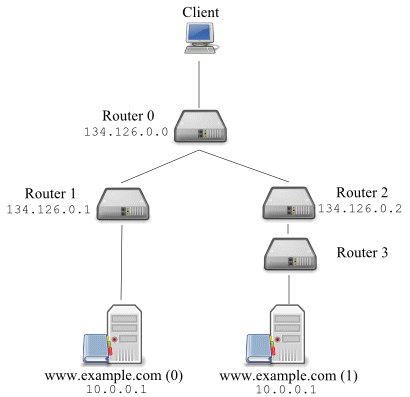
\includegraphics[width=0.5\linewidth]{images/anycast_slb}
		\caption{Beispiel eines Netzwerks aufgebaut mit Anycast}
		\label{anycast_slb_01}
	\end{center}
\end{figure}
\subsubsection{BGP Border Gateway Protcol}\cite{BGP}
Dieses Protokoll wird hauptsächlich im Internet eingesetzt und verbindet\textbf{ Autonome Systeme (AS)} miteinander. Ein AS kann man als eine große Anzahl von IP-Adressen, betrachtet als eine Einheit, ansehen. Das Protokoll verwendet für Routing-Entscheidungen sowohl strategische, wie auch technisch-metrische Kriterien, wobei in der Praxis zusätzlich betriebswirtschaftliche Aspekte berücksichtigt werden.

\subsubsection{Vorteile}
Der Vorteil bei diesem Verfahren ist die geographisch nahe Auswahl eines Servers mit entsprechender Verringerung der Latenz (Ping). Die Umsetzung erfordert allerdings die Instandhaltung eines eigenen Autonomen Systems



